\documentclass[10pt,letterpaper]{article}

\usepackage{iccv}
\usepackage{times}
\usepackage{epsfig}
\usepackage{graphicx}
\usepackage{amsmath}
\usepackage{amssymb}
\usepackage{makecell}
\usepackage{microtype}
\usepackage{footnote}
\usepackage{float}

\usepackage{siunitx} % apt install texlive-science
\sisetup
{
    exponent-to-prefix = true        ,
    round-mode         = places      ,
    round-precision    = 2           ,
    scientific-notation = engineering,
    zero-decimal-to-integer = false  ,
}

% Include other packages here, before hyperref.

% If you comment hyperref and then uncomment it, you should delete
% egpaper.aux before re-running latex.  (Or just hit 'q' on the first latex
% run, let it finish, and you should be clear).
\usepackage[pagebackref=true,breaklinks=true,letterpaper=true,colorlinks,bookmarks=false]{hyperref}
\usepackage{hypcap}

\iccvfinalcopy % *** Uncomment this line for the final submission

\def\iccvPaperID{1218} % *** TODO Enter the ICCV Paper ID here
\def\httilde{\mbox{\tt\raisebox{-.5ex}{\symbol{126}}}}

% Pages are numbered in submission mode, and unnumbered in camera-ready
\ificcvfinal\pagestyle{empty}\fi

\begin{document}

%\title{Copenhagen Skraafoto.
\title{Building Copenhagen in a Day\footnote{In 29 hours}.
\\ Supplementary Material for: \\ Out-of-Core Surface Reconstruction via Global $TGV$ Minimization.} % Replace with your title

\author{Nikolai Poliarnyi\\
    Agisoft LLC, St. Petersburg, Russia\\
    {\tt\small polarnick@agisoft.com}
}

\maketitle

In this supplementary, we want to show a public dataset with aerial photos of Copenhagen that we processed with our out-of-core surface reconstruction method.
Additionally, we provide closeups of the resulting model with per-vertex colors and breakdowns of other three datasets discussed in the paper -- see Tables~\ref{tab:citywall_breakdown}, ~\ref{tab:palacio_breakdown}, ~\ref{tab:tomb_breakdown}.

We downloaded 500 blocks (tiles) of photos covering \SI{425}{\km\squared} of the Copenhagen city from publicly available aerial photos of Denmark\footnote{\url{https://download.kortforsyningen.dk/content/skraafoto}} \cite{skraafoto_copenhagen}.
The downloaded blocks are shown in Fig.~\ref{fig:copenhagen_tiles}. For convenience, their names are also listed in the attached supplementary text file blocks.txt.
These 500 blocks (each covers \SI{1}{\km\squared}) contain 27472 aerial photos (566 GB) with resolutions of 13470x8670 and 10300x7700.
In addition to nadir photos, there is also oblique imagery -- one of such photos is shown in Fig.~\ref{fig:oblique_photo}.

For speedup, we downscaled these photos with a factor of 4 before running the SGM-based \cite{hirschmuller2007stereo} depthmap reconstruction.
This dataset was evaluated twice - on a small cluster of 7 affordable computers (on the average each computer was a PC with an 8-core CPU and a GeForce GTX 1080 GPU)
and on a single computer with an 8-core CPU and a GeForce GTX 1080 GPU.
The surface reconstruction took 29 hours on a small cluster of 7 computers, and the processing took 5.5 days on a single computer.
The breakdown of the processing on a cluster is shown in Table~\ref{tab:copenhagen_breakdown}.
The whole model with per-vertex color is shown in Fig.~\ref{fig:copenhagen_full_rgb}.

\begin{figure}[H]
    \centering
    \capstart
    \begin{minipage}[b]{0.45\linewidth}
        \includegraphics[width=\textwidth]{images/copenhagen/figures/tiles.png}
    \end{minipage}
    \begin{minipage}[b]{0.45\linewidth}
        \includegraphics[width=\textwidth]{images/copenhagen/figures/tiles_gmap.jpg}
    \end{minipage}
    \caption{Copenhagen dataset \cite{skraafoto_copenhagen}: 500 processed green blocks are shown (outlined with a blue border). To the right, a corresonding google map is shown \cite{gmaps_copenhagen}.}
    \label{fig:copenhagen_tiles}
\end{figure}

\begin{figure}[H]
    \centering
    \capstart
    \begin{minipage}[b]{1.0\linewidth}
        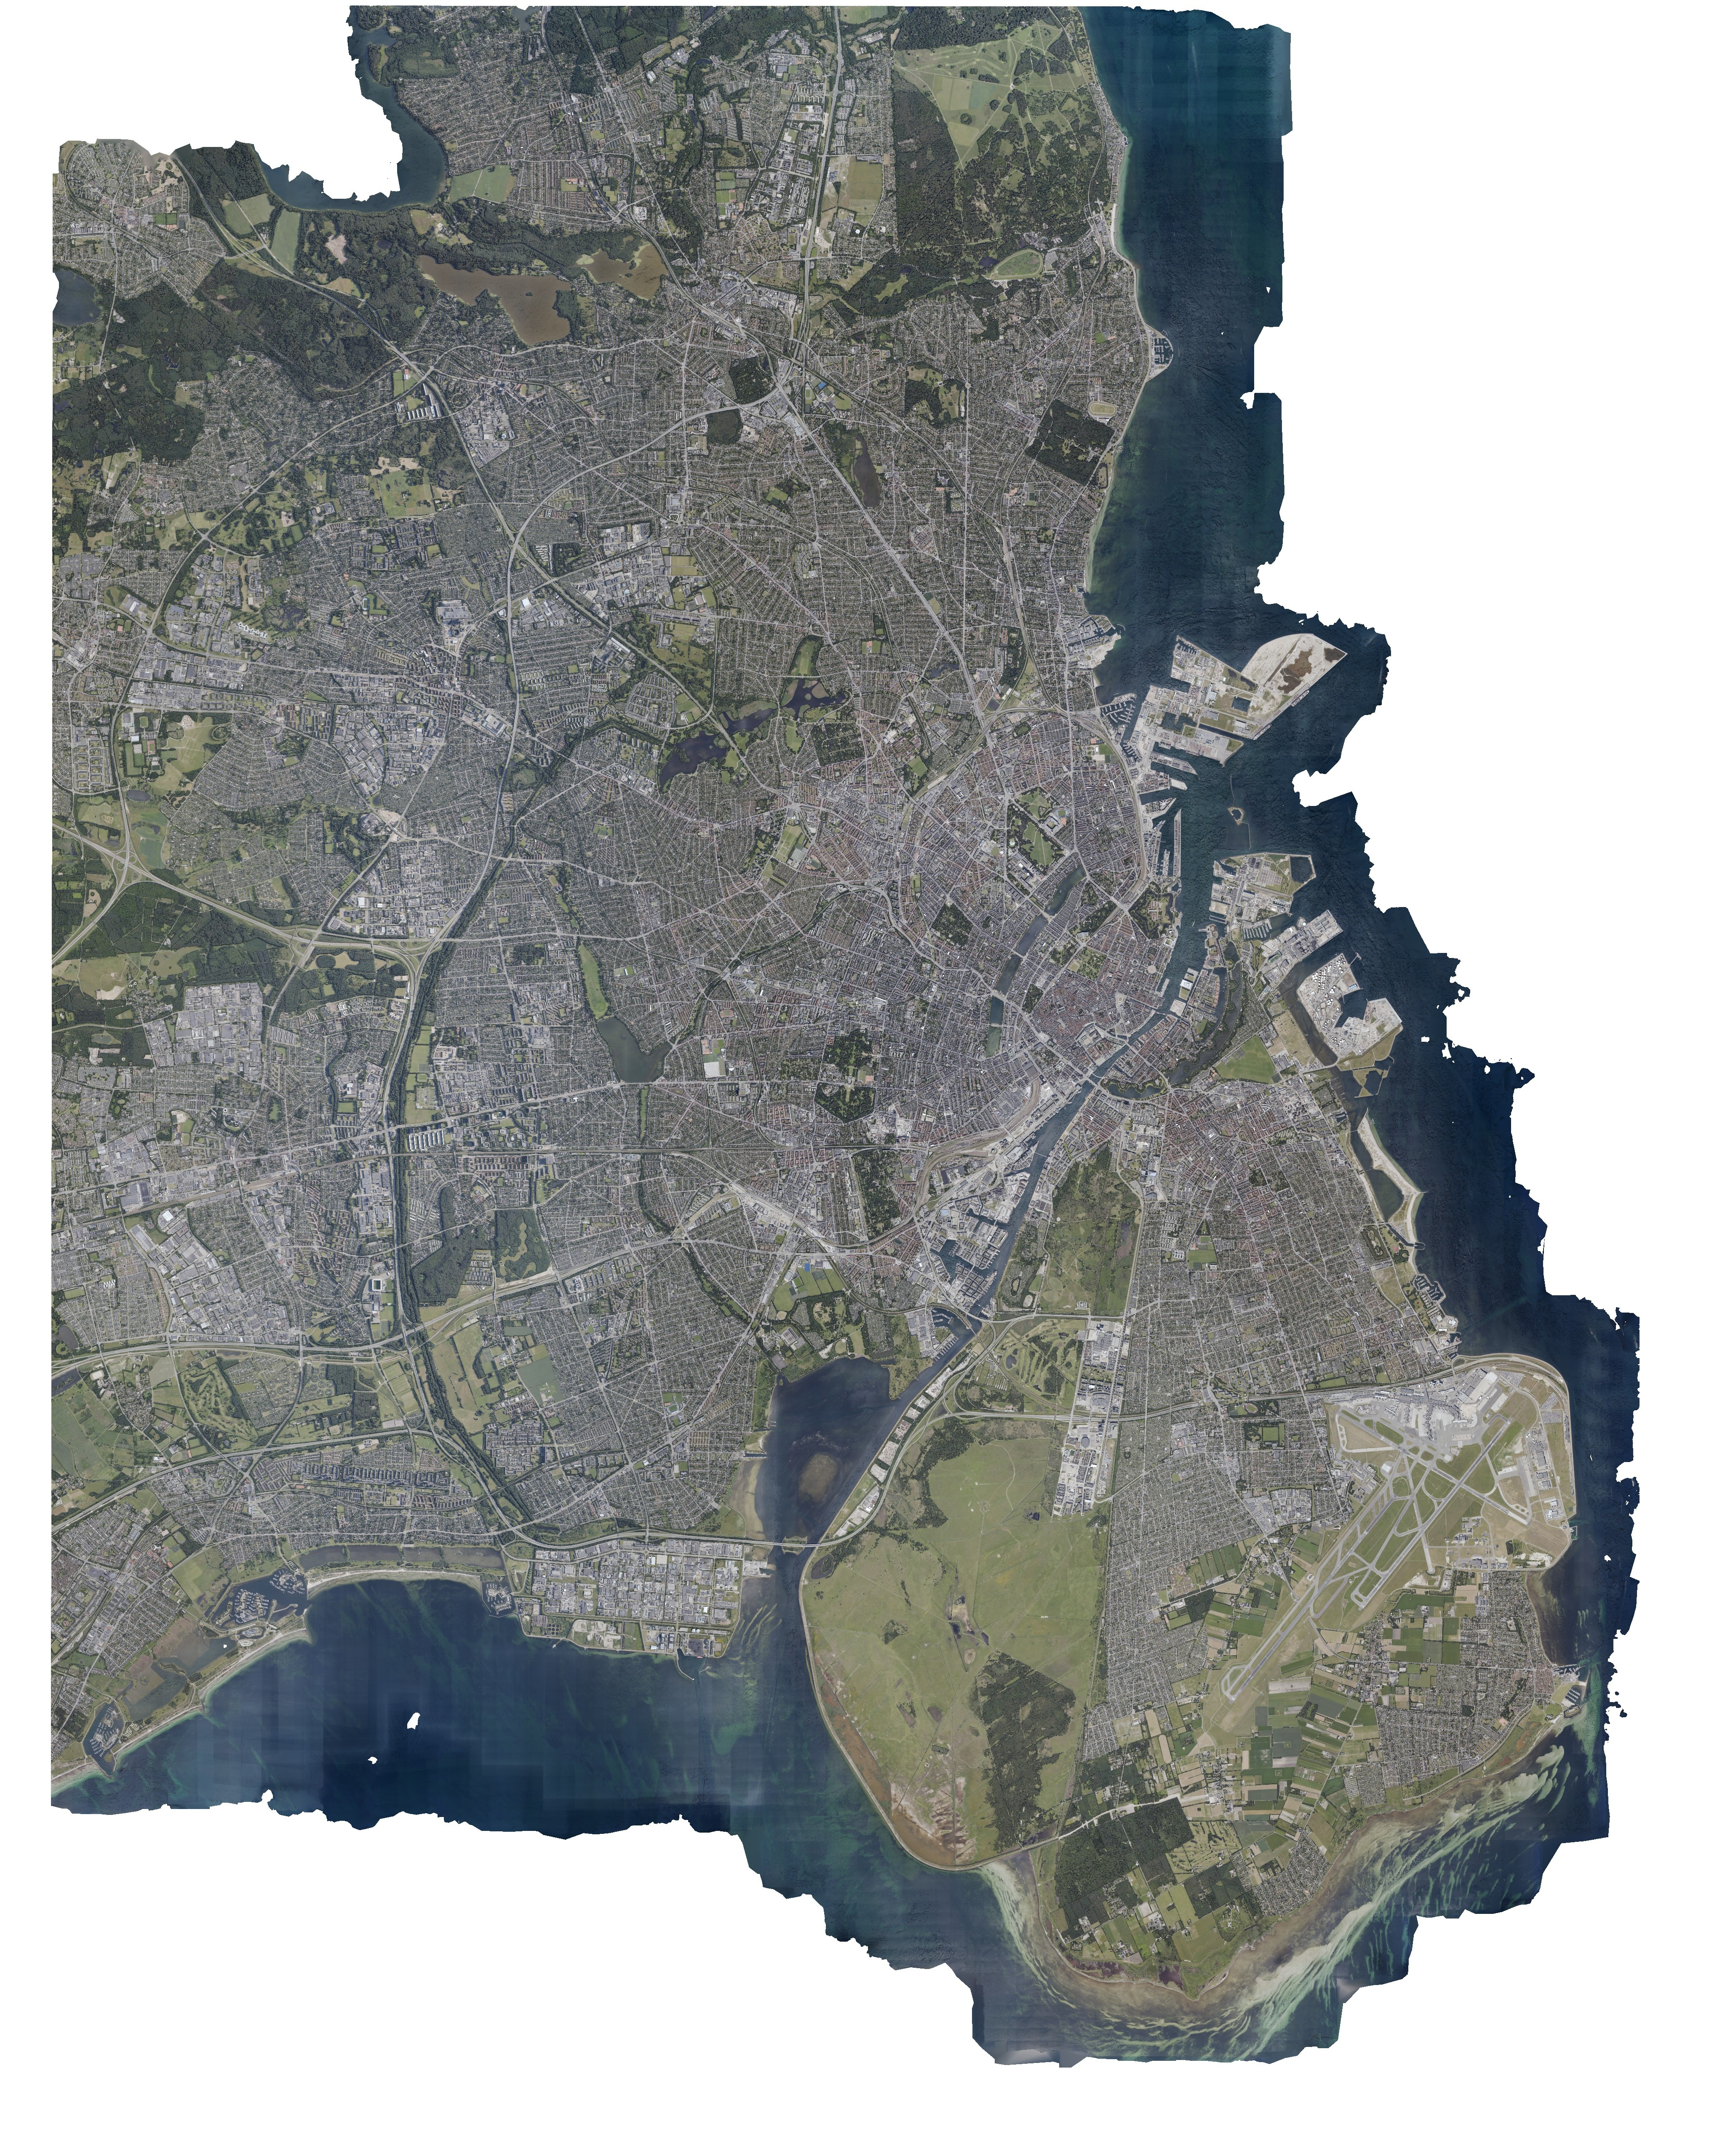
\includegraphics[width=\textwidth]{images/copenhagen/results/full/full_rgb.jpg}
    \end{minipage}
    \caption{Our method can handle an arbitrary large scene -- even \SI{425}{\km\squared} of the Copenhagen city.
    This polygonal model, consisting of 267 million triangles with per-vertex colors, was reconstructed from depth maps of 27472 aerial photos in 29 hours.}
    \label{fig:copenhagen_full_rgb}
\end{figure}

\begin{table*}

    \caption{
        A breakdown of the Copenhagen city dataset processing:
        27472 photos, 28 billion cubes from input depth maps, 29 hours of processing on a 7-computers cluster with the peak RAM usage -- 13.35 GB.
        %29:18%
    }

    \centering
    \begin{tabular*}{0.55\columnwidth}{  @{\extracolsep{\fill}} |l||c|c| @{} }
        \hline
        \textbf{Processing stage} & \textbf{Time} & \textbf{Time in \%} \\
        \hline
        %2020-03-08 01:01:45 - 03:54:49 - 06:23:49%
        Linear octree parts + merge & 173 + 149 min & 10\% + 8\% \\
        \hline
        %06:23:49 - 08:44:37 - 12:03:46%
        Balance octree parts + merge & 141 + 199 min & 8\% + 11\% \\
        \hline
        %12:03:46 - 13:23:40%
        Index treetop & 80 min & 5\%\\
        \hline
        %13:23:40 - 19:56:33%
        Histograms (GPU) & 393 min & 22\%\\
        \hline
        %19:56:33 - 22:35:19%
        Primal-dual method (GPU) & 159 min & 9\% \\
        \hline
        %22:35:19 - 06:00:24%
        Marching cubes & 445 min & 25\% \\
        \hline
    \end{tabular*}

    \label{tab:copenhagen_breakdown}

\end{table*}


\begin{table}

    \caption{
        A breakdown of the Citywall dataset processing:
        564 photos, 1205 million cubes from input depth maps, 63 minutes of processing on a computer with a 8-core CPU and a GeForce GTX 1080 GPU with the peak RAM usage -- 13.17 GB.
    }

    \centering
    \begin{tabular*}{0.55\columnwidth}{  @{\extracolsep{\fill}} |l||c|c| @{} }
        \hline
        \textbf{Processing stage} & \textbf{Time} & \textbf{Time in \%} \\
        \hline
        Linear octree + merge & 7 + 4 min & 10\% + 6\%\\
        \hline
        Balance octree + merge & 2 + 2 min & 3\% + 3\%\\
        \hline
        Index treetop & 2 min & 3\%\\
        \hline
        Histograms (GPU) & 17 min & 26\%\\
        \hline
        Primal-dual method (GPU) & 18 min & 28\% \\
        \hline
        Marching cubes & 12 min & 18\% \\
        \hline
    \end{tabular*}

    \label{tab:citywall_breakdown}

\end{table}

\begin{table}

    \caption{
        A breakdown of the Palacio Tschudi dataset processing:
        13703 photos, 16 billion cubes from input depth maps, 20 hours of processing on a computer with an 8-core CPU and a GeForce GTX 1080 GPU with the peak RAM usage -- 16.75 GB.
    }

    \centering
    \begin{tabular*}{0.55\columnwidth}{  @{\extracolsep{\fill}} |l||c|c| @{} }
        \hline
        \textbf{Processing stage} & \textbf{Time} & \textbf{Time in \%} \\
        \hline
        Linear octree + merge & 66 + 68 min & 5\% + 5\%\\
        \hline
        Balance octree + merge & 28 + 56 min & 2\% + 5\%\\
        \hline
        Index treetop & 32 min & 2\%\\
        \hline
        Histograms (GPU) & 370 min & 30\%\\
        \hline
        Primal-dual method (GPU) & 360 min & 30\% \\
        \hline
        Marching cubes & 240 min & 20\% \\
        \hline
    \end{tabular*}

    \label{tab:palacio_breakdown}

\end{table}

\begin{table}

    \caption{
        A breakdown of the Tomb of Tu Duc LIDAR dataset processing:
        42 LIDAR scans, 661 million cubes from input LIDAR scans, 160 minutes of processing on a computer with an 8-core CPU with a GeForce GTX 1080 GPU with peak RAM usage -- 10.05 GB.
    }

    \centering
    \begin{tabular*}{0.55\columnwidth}{  @{\extracolsep{\fill}} |l||c|c| @{} }
        \hline
        \textbf{Processing stage} & \textbf{Time} & \textbf{Time in \%} \\
        \hline
        Linear octree + merge & 4 + 3 min & 3\% + 2\%\\
        \hline
        Balance octree + merge & 5 + 21 min & 3\% + 13\%\\
        \hline
        Index treetop & 6 min & 4\%\\
        \hline
        Histograms (GPU) & 14 min & 9\%\\
        \hline
        Primal-dual method (GPU) & 54 min & 34\% \\
        \hline
        Marching cubes & 53 min & 33\% \\
        \hline
    \end{tabular*}

    \label{tab:tomb_breakdown}

\end{table}

\begin{figure}
    \centering
    \capstart
    \begin{minipage}[b]{0.32\linewidth}
        \includegraphics[width=\textwidth]{images/copenhagen/figures/2019_84_40_5_0034_00002391.jpg}
    \end{minipage}
    \begin{minipage}[b]{0.32\linewidth}
        \includegraphics[width=\textwidth]{images/copenhagen/figures/2019_84_40_5_0034_00002391_closeup1.jpg}
    \end{minipage}
    \begin{minipage}[b]{0.32\linewidth}
        \includegraphics[width=\textwidth]{images/copenhagen/figures/2019_84_40_5_0034_00002391_closeup2.jpg}
    \end{minipage}
    \caption{Example of oblique photo with resolution 7700x10300. skraa\_1km\_6168\_720\_JPG\_UTM32-ETRS89.zip / 2019\_84\_40\_5\_0034\_00002391.jpg}
    \label{fig:oblique_photo}
\end{figure}

\begin{figure}
    \centering
    \capstart
    \begin{minipage}[b]{1.0\linewidth}
        \includegraphics[width=\textwidth]{images/copenhagen/results/closeups/diag/frederiksberg_forsyning_as_diag.jpg}
    \end{minipage}
    \caption{Frederiksberg Forsyning A/S closeup. Note that both pipes were reconstructed well.}
    \label{fig:closeup_frederiksberg}
\end{figure}

\begin{figure}
    \centering
    \capstart
    \begin{minipage}[b]{1.0\linewidth}
        \includegraphics[width=\textwidth]{images/copenhagen/results/closeups/diag/banedanmark_diag.jpg}
    \end{minipage}
    \caption{Banedanmark closeup.}
    \label{fig:closeup_banedanmark}
\end{figure}

\begin{figure}
    \centering
    \capstart
    \begin{minipage}[b]{1.0\linewidth}
        \includegraphics[width=\textwidth]{images/copenhagen/results/closeups/diag/avedore_power_station_diag.jpg}
    \end{minipage}
    \caption{Aved{\o}re Power Station closeup. Note accurate geometry of thin structures above the ground.}
    \label{fig:closeup_power_station}
\end{figure}

\begin{figure}
    \centering
    \capstart
    \begin{minipage}[b]{1.0\linewidth}
        \includegraphics[width=\textwidth]{images/copenhagen/results/closeups/diag/airport_diag.jpg}
    \end{minipage}
    \caption{Airport closeup.}
    \label{fig:closeup_airport}
\end{figure}

\begin{figure}
    \centering
    \capstart
    \begin{minipage}[b]{1.0\linewidth}
        \includegraphics[width=\textwidth]{images/copenhagen/results/closeups/diag/hofor_as_diag.jpg}
    \end{minipage}
    \caption{Hofor Amagerverket closeup.}
    \label{fig:closeup_hofor}
\end{figure}

\begin{figure}
    \centering
    \capstart
    \begin{minipage}[b]{1.0\linewidth}
        \includegraphics[width=\textwidth]{images/copenhagen/results/closeups/diag/christiansborg_palace_diag.jpg}
    \end{minipage}
    \caption{Christiansborg Palace closeup.}
    \label{fig:closeup_christiansborg_palace}
\end{figure}

\begin{figure}
    \centering
    \capstart
    \begin{minipage}[b]{1.0\linewidth}
        \includegraphics[width=\textwidth]{images/copenhagen/results/closeups/diag/kastellet_diag.jpg}
    \end{minipage}
    \caption{Kastellet closeup.}
    \label{fig:closeup_kastellet}
\end{figure}

\begin{figure}
    \centering
    \capstart
    \begin{minipage}[b]{1.0\linewidth}
        \includegraphics[width=\textwidth]{images/copenhagen/results/closeups/diag/frederiks_church_diag.jpg}
    \end{minipage}
    \caption{Frederik's Church closeup.}
    \label{fig:closeup_frederik_church}
\end{figure}

\begin{figure}
    \centering
    \capstart
    \begin{minipage}[b]{1.0\linewidth}
        \includegraphics[width=\textwidth]{images/copenhagen/results/closeups/diag/rosenborg_castle_diag.jpg}
    \end{minipage}
    \caption{Rosenborg Castle closeup.}
    \label{fig:closeup_rosenborg_castle}
\end{figure}

\begin{figure}
    \centering
    \capstart
    \begin{minipage}[b]{1.0\linewidth}
        \includegraphics[width=\textwidth]{images/copenhagen/results/closeups/diag/herlev_hospital_diag.jpg}
    \end{minipage}
    \caption{Herlev Hospital closeup.}
    \label{fig:closeup_hospital}
\end{figure}

\begin{figure}
    \centering
    \capstart
    \begin{minipage}[b]{1.0\linewidth}
        \includegraphics[width=\textwidth]{images/copenhagen/results/closeups/diag/hotel_marriott_bella_sky_diag.jpg}
    \end{minipage}
    \caption{AC Hotel by Marriott Bella Sky closeup.}
    \label{fig:closeup_hotel}
\end{figure}

\begin{figure}
    \centering
    \capstart
    \begin{minipage}[b]{1.0\linewidth}
        \includegraphics[width=\textwidth]{images/copenhagen/results/closeups/diag/telia_parken_diag.jpg}
    \end{minipage}
    \caption{Telia Parken Stadium closeup.}
    \label{fig:closeup_stadium}
\end{figure}

\begin{figure}
    \centering
    \capstart
    \begin{minipage}[b]{1.0\linewidth}
        \includegraphics[width=\textwidth]{images/copenhagen/results/closeups/diag/rigshospitalet_diag.jpg}
    \end{minipage}
    \caption{Rigshospitalet closeup.}
    \label{fig:closeup_rigshospitalet}
\end{figure}

\begin{figure}
    \centering
    \capstart
    \begin{minipage}[b]{1.0\linewidth}
        \includegraphics[width=\textwidth]{images/copenhagen/results/closeups/diag/un_city_diag.jpg}
    \end{minipage}
    \caption{UN City closeup.}
    \label{fig:closeup_un_city}
\end{figure}

\begin{figure}
    \centering
    \capstart
    \begin{minipage}[b]{1.0\linewidth}
        \includegraphics[width=\textwidth]{images/copenhagen/results/closeups/diag/mountain_dwellings_diag.jpg}
    \end{minipage}
    \caption{Mountain Dwellings closeup.}
    \label{fig:closeup_mountain_dwellings}
\end{figure}

\clearpage
{\small
\bibliographystyle{ieee_fullname}
\bibliography{egbib}
}

\end{document}
